\documentclass[border=3mm,tikz,preview]{standalone}
\usepackage[utf8]{inputenc}
\usepackage{amsmath,amssymb,amsfonts}
\usepackage{graphicx}
\usepackage{tikz}
\usetikzlibrary{shapes.geometric, arrows.meta, positioning, shadows, calc, fit, backgrounds}
\usepackage{xcolor}
\begin{document}

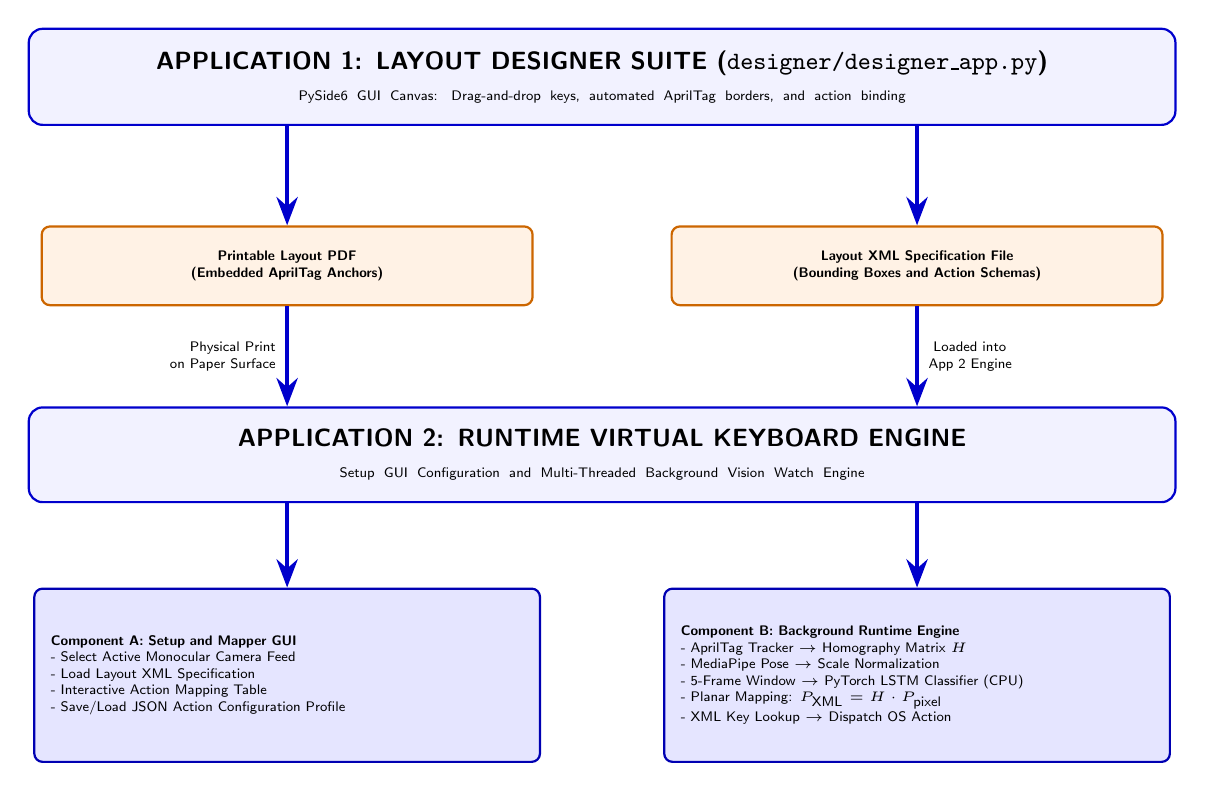
\begin{tikzpicture}[
    appbox/.style = {rectangle, draw=blue!80!black, fill=blue!5!white, thick, rounded corners=5pt, align=center, font=\sffamily\bfseries\small, inner sep=8pt, text width=14cm},
    compbox/.style = {rectangle, draw=blue!70!black, fill=blue!10!white, thick, rounded corners=3pt, align=left, font=\sffamily\tiny, inner sep=6pt, text width=6.0cm, minimum height=2.2cm},
    artbox/.style = {rectangle, draw=orange!80!black, fill=orange!10!white, thick, rounded corners=3pt, align=center, font=\sffamily\bfseries\tiny, text width=6.0cm, minimum height=1.0cm},
    arrow/.style = {draw=blue!80!black, ->, >=Stealth, ultra thick}
]

% Tier 1: Application 1
\node (app1) [appbox] at (0, 0) {
\textbf{APPLICATION 1: LAYOUT DESIGNER SUITE (\texttt{designer/designer\_app.py})}\\
{\normalfont\sffamily\tiny PySide6 GUI Canvas: Drag-and-drop keys, automated AprilTag borders, and action binding}
};

% Tier 2: Synchronized Artifacts (x = -4.0 and x = +4.0)
\node (pdf_art) [artbox] at (-4.0, -2.4) {Printable Layout PDF\\(Embedded AprilTag Anchors)};
\node (xml_art) [artbox] at (4.0, -2.4) {Layout XML Specification File\\(Bounding Boxes and Action Schemas)};

% Tier 3: Application 2 Container
\node (app2) [appbox] at (0, -4.8) {
\textbf{APPLICATION 2: RUNTIME VIRTUAL KEYBOARD ENGINE}\\
{\normalfont\sffamily\tiny Setup GUI Configuration and Multi-Threaded Background Vision Watch Engine}
};

% Tier 4: Application 2 Subcomponents (x = -4.0 and x = +4.0)
\node (comp_a) [compbox] at (-4.0, -7.6) {
\textbf{Component A: Setup and Mapper GUI}\\
- Select Active Monocular Camera Feed\\
- Load Layout XML Specification\\
- Interactive Action Mapping Table\\
- Save/Load JSON Action Configuration Profile
};

\node (comp_b) [compbox] at (4.0, -7.6) {
\textbf{Component B: Background Runtime Engine}\\
- AprilTag Tracker $\to$ Homography Matrix $H$\\
- MediaPipe Pose $\to$ Scale Normalization\\
- 5-Frame Window $\to$ PyTorch LSTM Classifier (CPU)\\
- Planar Mapping: $P_{\text{XML}} = H \cdot P_{\text{pixel}}$\\
- XML Key Lookup $\to$ Dispatch OS Action
};

% Perfectly vertical, aligned connections (no diagonal crossing, no piercing boxes)
\draw [arrow] (app1.south -| pdf_art.north) -- (pdf_art.north);
\draw [arrow] (app1.south -| xml_art.north) -- (xml_art.north);

\draw [arrow] (pdf_art.south) -- node[left, font=\sffamily\tiny, align=right]{Physical Print\\on Paper Surface\ } (app2.north -| pdf_art.south);
\draw [arrow] (xml_art.south) -- node[right, font=\sffamily\tiny, align=left]{\ Loaded into\\App 2 Engine} (app2.north -| xml_art.south);

\draw [arrow] (app2.south -| comp_a.north) -- (comp_a.north);
\draw [arrow] (app2.south -| comp_b.north) -- (comp_b.north);

\end{tikzpicture}

\end{document}
